% !TEX root = ../main.tex
\chapter{Dependency evaluation model}\label{ch:TheoreticModel}



\section{Definition of coupling (RQ1.1)}\label{section:defCoupling}
% IMPORTANT: Difference between direct and indirect coupling. Detecting Indirect Coupling Yang et al. 2005
To measure the degree of dependency, we are going to define the characteristics of the coupling of the dependencies with a project. Following the six criteria in the framework defined by Briand et al. \cite{briand1999unified}, described in Section \ref{section:bg-coupling}, we are going to define the coupling to measure.

\paragraph{Criterion 1 - Type of connection:}
With this criterion, it is defined which type of connection creates coupling between the two items, previously defined as two separate sets of classes. There are several and clearly distinguished mechanisms that can create coupling, as defined by Briand et al. \cite{briand1999unified}, listed below.

\blankls
Given class \textit{a} of set of classes \textit{A}, and class \textit{b} of set of classes \textit{B}...

\begin{enumerate}
  \item ... class \textit{a} has an attribute of type \textit{b} (Relationship of aggregation).
  \item ... method of class \textit{a} has a parameter of type \textit{b} or has return type \textit{b}.
  \item ... method of class \textit{a} has a local variable of type \textit{b}.
  \item ... method of class \textit{a} calls a method which has a parameter of type \textit{b}.
  \item ... method of class \textit{a} references attribute of class \textit{b}.
  \item ... method of class \textit{a} invokes method of class \textit{b}.
  \item ... class \textit{a} and class \textit{b} have a relationship such as uses or consists-of.
\end{enumerate}

Having one metric measure more than one of these types of connections is not recommended, for a variety of reasons. To begin with, the strengths of every type of connection have to be justified: Has one connection of type 5 the same strength as a connection of type 6? Also, when mixing types of connection there is information missing, it is not possible to know how much of the coupling is created by which connection. Therefore, all relevant types of connections in the use case of RQ1 are going to be measured by different metrics.

To decide which types of connections to measure, %since all of them create coupling between libraries,
we have decided to review the literature on coupling metrics, to understand which connections are the most measured and why.

\begin{table}[ht!]
    \centering
    \begin{tabular}{|l|c|c|c|c|c|c|c|}
         \hline
         Reference                      & 1 & 2 & 3 & 4 & 5 & 6 & 7 \\\hline
         \cite{eder1994coupling}        & x & x & x & x &   & x & x \\\hline
         \cite{hitz1995measuring}       & x & x & x &   & x & x & x \\\hline
         \cite{briand1997investigation} & x & x &   &   &   & x &   \\\hline
         \cite{wilkie2000coupling}      & x & x &   &   &   &   &   \\\hline
         \cite{yang2005detecting}       & x & x & x & x &   & x &   \\\hline
         \cite{gui2007ranking}          & x &   &   &   & x & x &   \\\hline
         \cite{gupta2009package}        & x & x & x & x & x & x & x \\\hline
         \cite{harrison1998coupling}    &   &   &   &   & x & x &   \\\hline
         \cite{du2004refactoring}       & x &   &   &   & x & x &   \\\hline
         \cite{koetter2019assessing}    & x &   &   &   & x & x &   \\\hline
    \end{tabular}
    \caption{Literature usage of the types of connection}
    \label{tab:type-con-literature}
\end{table}

 Types 1 and 6 are the most used in the literature and therefore we define a metric to measure \textbf{type 6: method invocation}.

The second metric that we consider is \textbf{type 1: aggregation coupling}, for two main reasons. It is used as type 6 in the reviewed literature, and because in some cases, measuring type 6 may not be enough to understand how much maintenance a library dependency may need. There is the possibility that a class has an attribute of another class, but never calls a method that belongs to that class.

% Change this when the set of metrics is final
The above-mentioned metrics are those that we initially consider in our work, and we will explain them in greater detail in Section~\ref{section:defMetrics}. Nevertheless, it might be necessary to include additional metrics, to account for other connection types.

\paragraph{Criterion 2 - Locus of impact:}
As explained in section \ref{section:bg-coupling}, Briand et al. propose two options for the locus of impact: import and export. According to the definition of the problem, the goal of this measurement is to know how much a library depends on another. Therefore, the point of view of this evaluation is from the library that uses another one. Hence, the locus of impact of the coupling to be measured in this thesis is \textbf{import}. We measure the dependency from the point of view of the library that acts as a client of a server library.

\paragraph{Criterion 3 - Granularity of the measure:}
In this criterion, there are two aspects to define. (1) The aggregation level of the measure, and (2) how the metric counts the connections. First, we are going to discuss the domain level. Briand et al. define the following levels:

\begin{itemize}[noitemsep]
  \renewcommand\labelitemi{--}
  \item Attribute
  \item Method
  \item Class
  \item Set of classes
  \item System
\end{itemize}

\blankls
In this case, the goal is to measure the coupling between the set of classes of the client library and the set of classes of the server library. The measurement is done by aggregating the coupling of the more fine-grained levels \cite{briand1999unified}. For consistency, we are going to name the aggregation level \textbf{library level}.

Next, we define how the metric has to count connections. The options for counting connections defined by Briand et al. are explained in section \ref{section:bg-coupling}, in Table \ref{table:counting-connections}. The options B), D), E), and F), are not useful for this research. These options count the distinct items at the other end of the connection, not considering how many times those items are at the other end of the connection.

The two other options are A) and C), which count individual connections. The difference between A and C is the aggregation level at which the connections are counted. The option C) counts the connections as in A), but adding up the result for each method or attribute of a class. Since the level of the domain of the metrics is not class but set of classes, a new option for counting connections is defined. The definition is created following the same style as Briand et al.: \textbf{Add up the number of connections counted as in C) for each class of the set of classes}. By following this method of aggregating the number of connections through aggregation levels, a fine-grained analysis is maintained for the aggregation level of the metrics.

\paragraph{Criterion 4 - Stability of the server:}
Following the definition of stability stated by Briand et al. \cite{briand1999unified}, in this case, the server has to be stable. Briand et al. define stable classes as \textit{"Classes that are not subject to change in the project at hand"}. Therefore, we are going to count connections from non-stable classes to \textbf{stable classes}. According to the previously defined locus of impact, the non-stable classes are the clients of the stable classes.

However, in the use case of this thesis, the differentiation between stable and unstable classes is not enough. The goal is to measure coupling only with classes that are part of other open-source libraries. Therefore, the classes that belong to standard libraries and the programming language types, although being stable classes, will not be considered by the metrics.

\paragraph{Criterion 5 - Direct and indirect coupling:}
To decide which option we want to define for this criterion, we need to distinguish two alternative scenarios in which we want to measure coupling: Direct dependencies and transitive dependencies. When measuring direct dependencies, we want to measure only direct coupling between the sets of classes, whereas for transitive dependencies it is necessary to measure indirect coupling. Hence, \textbf{both types of coupling} will be measured, with two different metrics for each type of connection relevant for this case: One for direct dependencies and another one for transitive dependencies.

\paragraph{Criterion 6 - Inheritance:}
Within this criterion, there are three aspects to decide about: how, if at all, does the metric distinguish between inheritance-based coupling and noninheritance-based coupling? If the metric counts method invocations, does it account for polymorphism? And finally, what defines if a method is part of a class or not?

\begin{figure}[ht]
\begin{center}
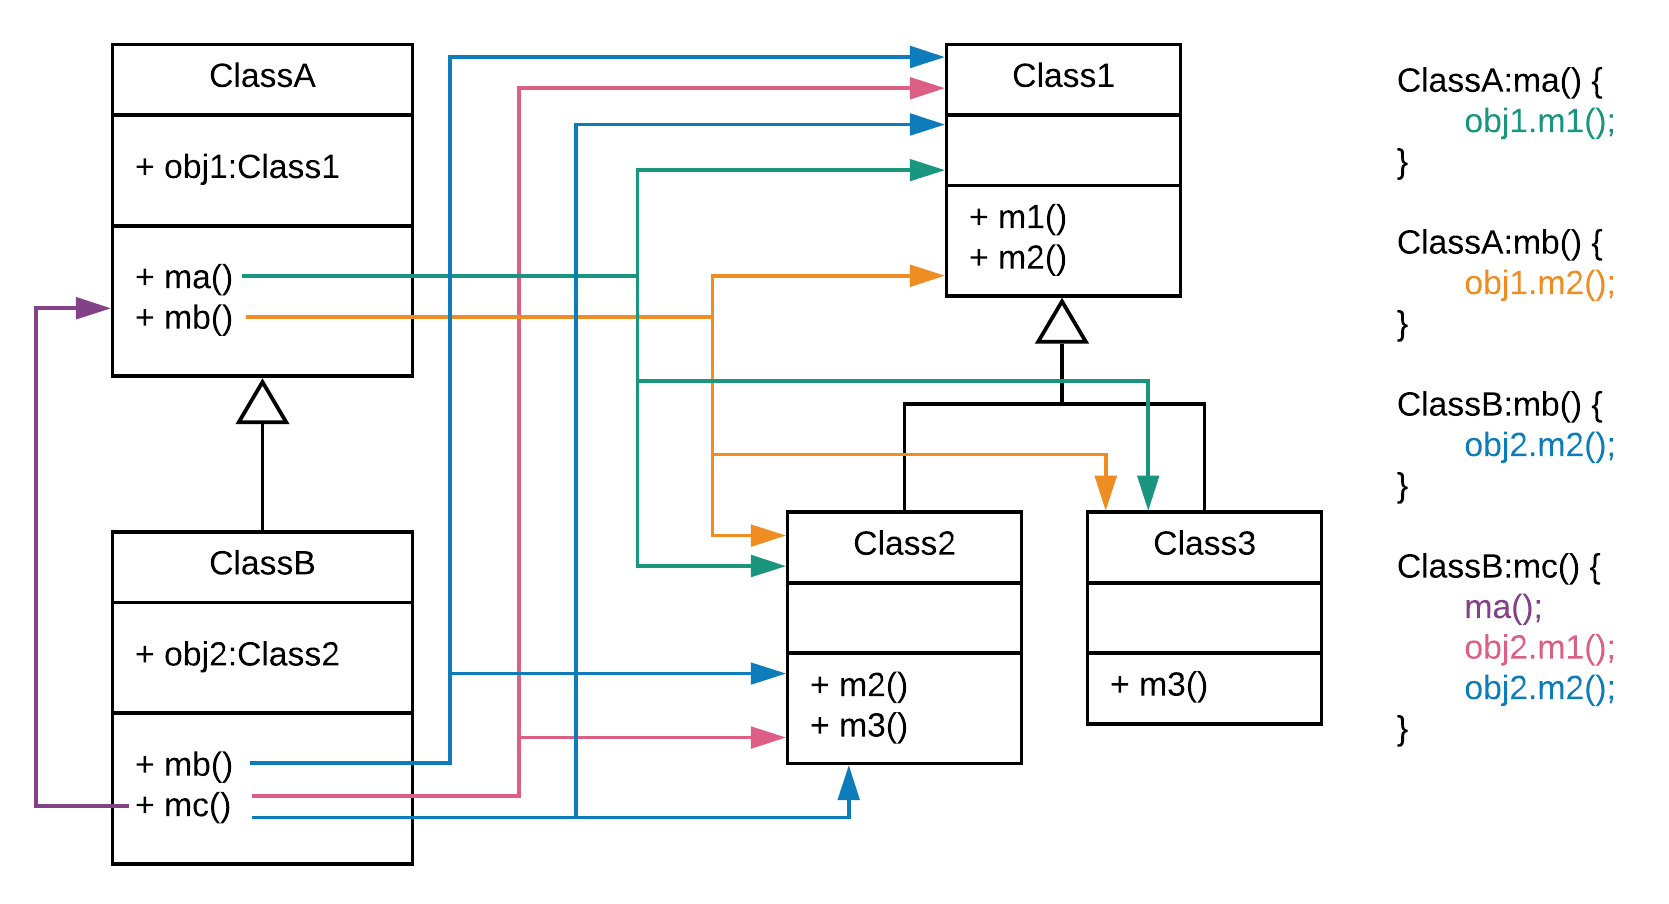
\includegraphics[width=\textwidth]{figures/specialcases.png}
\caption{Example of coupling special cases, based on example from Briand et al. \cite{briand1999unified}}
\label{fig:specialcases}
\end{center}
\end{figure}

In order to answer the first question, we focus on the method \texttt{mc} of \texttt{ClassB} in Figure \ref{fig:specialcases}. This method invokes \texttt{ma} of \texttt{ClassA}, inherited by \texttt{ClassB}.

This is known as \textit{inheritance-based} coupling is sometimes considered as a special case of coupling.
When there is a change of an inherited method that a class uses, it  requires the same maintenance effort as the method that is not inherited. Therefore, our metrics  \textbf{include inheritance-based coupling without distinction}.

% Next, we discuss about whether to account for polymorphism.
In the case of the second question, polymorphism, we look at the methods of \texttt{ClassA}. This class contains an attribute of type \texttt{Class1}, which considering dynamic assignation of types could also be of type \texttt{Class2} or \texttt{Class3}.
%In this case,
We first analyze whether a call to a method of \texttt{Class1} would create coupling with \texttt{Class2} and \texttt{Class3}, and if it makes a difference when the method is overridden or not. The method \texttt{ma} invokes \texttt{m1}, which is not overridden by any of the descendants of \texttt{Class1}. When a change is made in \texttt{Class2} or \texttt{Class3} no change is required as the invoked method remains the same. In contrast, method \texttt{mb} calls \texttt{m2}, which is overridden in \texttt{Class2}. Here, the implementation of \texttt{m2} in \texttt{Class2} could be updated, and this may affect the way \texttt{ClassA} uses it, and therefore changes may be needed. Thus, it is necessary to \textbf{account for polymorphism}.

Lastly, we discuss about how do decide if a method belongs or not to a class. We have two options: (1) a method belongs to the class that implements it (could be more than one since we account for polymorphism), or (2) a method belongs to the class that it is referenced from. An example of this can be found in the last two lines of the method \texttt{mc} of \texttt{ClassB} call method \texttt{m1} and \texttt{m2} on an object of type \texttt{Class2}. The difference is that \texttt{m1} is implemented in \texttt{Class1} and \texttt{m2} is overridden in \texttt{Class2}. From a maintenance perspective, when the method \texttt{m1} is updated in \texttt{Class1}, this probably requires update in \texttt{ClassB} as well. However, changes in \texttt{Class2} will not generate a need to update the method call in \texttt{ClassB}. When  \texttt{m2} is updated in \texttt{Class1}, it will not make a difference for this call to \texttt{m2} since it is not executing the implementation of \texttt{Class1}. Therefore, \textbf{a method call creates coupling with the class that contains the implementation}.



\paragraph{Result}
All the metrics that are going to be used to measure the dependencies between libraries, are classified in Table \ref{table:metric-characteristics} according to the previous discussion on the criteria.

\begin{table}[h]
    \begin{center}
    \begin{tabular}{|l|l|l|l|l|l|l|l|l|}
    \hline
    \rot{Metric} & \rot{Type of connection} & \rot{Locus of impact} & \rot{Domain of measure} & \rot{Counting connections   } & \rot{Direct/Indirect} & \rot{Inheritance} & \rot{Polymorphism} & \rot{Item belongs to class} \\ \hline
    \hline
    \#1   & 6 & Import & Library & G & Direct   & Both, no distinction & Yes & Implemented \\\hline
    \#2   & 1 & Import & Library & G & Direct   & Both, no distinction & Yes & Implemented \\\hline
    \hline
    \#3   & 6 & Import & Library & G & Indirect & Both, no distinction & Yes & Implemented \\\hline
    \#4   & 1 & Import & Library & G & Indirect & Both, no distinction & Yes & Implemented \\\hline
    \end{tabular}
    \end{center}
    \caption{Criteria of the set of metrics}
    \label{table:metric-characteristics}
\end{table}

\section{Metrics for direct dependencies}

\subsection{Formal definition of the metrics (RQ1.2)}\label{section:defMetrics}
In this section, there is the formulation of the formal definition of the metrics. However, before the definitions, there is a brief discussion in which the definition of coupling of the proposed metrics are compared with the existing metrics in the literature described in Section \ref{section:bg-coupling}.

\subsubsection{Revisiting existing metrics}
Once we have defined the coupling that is going to be measured by each of the metrics, we can compare it with the existing coupling metrics, according to Table \ref{table:coupling-metrics} in Section \ref{section:bg-coupling}.

\paragraph{Metric 1}
To compare the coupling defined for metric 1 with the existing metrics, we focus on the metrics with the following characteristics:

\begin{itemize}
  \item Type of connection: 6, method invocations
  \item Locus of impact: import
  \item Direct or indirect coupling: direct
  \item Counting connections: count individual connections (option A or C).
\end{itemize}

The metrics that share these characteristics are \textit{MPC}, the group \textit{ICP}, and the metrics \textit{AMMIC}, \textit{IFMMIC} and \textit{OMMIC} from the suite of metrics by Briand et al.. However, \textit{MPC} does not consider polymorphic implementations of the called methods. \textit{IFMMIC} is a metric formulated specifically for C++ \cite{briand1997investigation} and therefore is not useful for our model.

From the group of metrics \textit{ICP}, the metric \textit{ICP}  considers both inheritance and non-inheritance coupling and therefore shares the definition of coupling with our metric 1. Nevertheless, according to the definition of \textit{ICP}, the coupling created by each method call is weighted by the number of parameters of the called method. In this aspect, it differs from metric 1.

Finally, the metrics \textit{AMMIC} and \textit{OMMIC} use the same definition of coupling as metric 1 except that \textit{AMMIC} counts the method invocations to ancestors and \textit{OMMIC} to other classes. Therefore, metric 1 is the sum of \textit{AMMIC} and \textit{OMMIC} but aggregated to the library aggregation level instead of class level.

\paragraph{Metric 2}
In the case of metric 2, we focus on the metrics with the following characteristics:

\begin{itemize}
  \item Type of connection: 1, client class contains an attribute of type server class, aggregation coupling
  \item Locus of impact: import
  \item Direct or indirect coupling: direct
  \item Counting connections: count individual connections (option A or C)
\end{itemize}

According to Table \ref{table:coupling-metrics}, the metrics that share these characteristics are \textit{DAC}, and from the suite of metrics by Briand et al. the metrics \textit{IFCAIC}, \textit{ACAIC} and \textit{OCAIC}. However, \textit{IFCAIC} is an extension for C++ and will not be considered.

According to the definition of \textit{DAC}, it counts the number of attributes of a class that have any other class as type. Therefore, instead of calculating the coupling between two classes, it calculates the coupling of a class with every other class. However, metric 2 is used at the library level, and to calculate coupling between two libraries instead of the coupling of one library with all the others.

Finally, \textit{ACAIC} and \textit{OCAIC} consider aggregation coupling with ancestors and others respectively. Therefore, metric 2 is the sum of these two metrics, but aggregated to library aggregation level, since the metrics are designed for class level.

\subsubsection{Formal definition}\label{subsec:metric-definition}
\paragraph{Metric 1: Direct method invocation coupling (MIC)}
The $\verb|MIC|$ metric measures the dependency between two libraries, one acting as client ($L_c$) and the other as server ($L_s$).%, based on the method invocations from $L_c$ to $L_s$.
Based on the criterion 3 discussed in Section~\ref{section:defCoupling}, this metric is calculated for each of the classes implemented in $L_c$, and for each of the methods implemented $\verb|M|(L_c)$ in these classes. For each implemented method  $m_c \in \verb|M|(L_c)$, we count the number of individual invocations to a method of $L_s$, denoted $\verb|nII|(m_c,L_s)$. For each method invocation made by the methods implemented in $L_c$, we count only the ones that are implemented in stable classes (not implemented in $L_c$). The set of stable methods invoked is denoted $\verb|SIM|(m_c)$.

\begin{equation*}
\verb|MIC|(L_c, L_s) =\!\!\!\!\! \sum_{m_c \in \verb|M|(L_c)} \verb|nII|(m_c, L_s)
\end{equation*}

According to criterion 6, it is necessary to take into account all the polymorphic implementations of the invoked method that are implemented in $L_s$. Therefore, we intersect the set of polymorphic implementations of an invoked method $\verb|PM|(m_s)$ with the set of methods $\verb|M|(L_s)$ implemented in $L_s$. Finally, to obtain the number of individual invocations, $\verb|nII|(m_c,L_s)$, we multiply the number of times a stable method ($m_s \in \verb|SIM|(m_c)$) has been invoked, $\verb|nI|(m_c, m_s)$ by the number of polymorphic implementations $\verb|nP|(m_s, L_s)$ of the method in $L_s$.

\begin{equation*}
   \verb|nII|(m_c, L_s) =\!\!\! \sum_{m_s \in \verb|SIM|(m_c)} \verb|nI|(m_c, m_s)*\verb|nP|(m_s, L_s)
\end{equation*}

\begin{equation*}
    \verb|nP|(m_s, L_s) = |\verb|PM|(m_s) \cap \verb|M|(L_s)|
\end{equation*}

\paragraph{Metric 2: Direct aggregation coupling (AC)}
%The process for this metric is similar to the one of the first metric. However, in this case,
The $\verb|AC|$ metric counts the number of times when a class of $L_c$ has an attribute whose type is a class implemented in $L_s$. Therefore, the metric is calculated for each class implemented in $L_c$ ($\verb|C|(L_c)$). For each class, we consider only those attributes types that are stable classes (not implemented in $L_c$). The set of stable attribute types in a class $c$ %that are stable
is $\verb|SAT(c_c)|$.

%According to criterion 6, in this case,
To account for polymorphism (criterion 6), we count all the descendants of the class that are implemented in $L_s$. Therefore, we intersect the set %with the descendants of the class, $\verb|DC|(c_s)$, with the set of
of the class descendants, $\verb|DC|(c_s)$, with the set of
classes implemented in $L_s$ ($\verb|C|(L_s)$). Finally, to count the  individual connections, we multiply the number of times a client class $c_c$ has an attribute of type the server class $c_s$ $\verb|NA|(c_c, c_s)$ by the number of class descendants (class included) implemented in $L_s$ ($\verb|nDC|(c_s,L_s)$).

\begin{equation*}
  \verb|AC|(L_c,L_s) = \!\!\!\!\sum_{c_c \in \verb|C|(L_c)} \sum_{c_s \in \verb|SAT|(c_c)} \!\!\!\!\verb|NA|(c_c, c_s)*\verb|nDC|(c_s, L_s)
\end{equation*}

\begin{equation*}
    \verb|nDC|(c_s, L_s) = |\verb|DC|(c_s) \cap \verb|C|(L_s)|
\end{equation*}

\subsection{Theoretical validation (RQ1.5)}
The theoretical validation of the metrics consists of demonstrating the properties of the metrics. The theoretical validation is necessary since it proves that the metrics share some properties with the attribute these are measuring, in this case coupling. In particular, for coupling metrics there are five properties defined by Briand et al. \cite{briand1996property} which have been largely used by the literature \cite{poshyvanyk2006conceptual, allen1999measuring, zhao2004measuring}.

For the description of the properties, we use $Coupling(L_c, L_s)$ to refer to any of the metrics defined in the previous section. The description of the metrics is based on the description done by Briand et al. which was done for coupling metrics that measure the coupling within an element, or coupling between an element and all the other elements with which it has some type of relationship. Therefore, the description has been adapted for coupling metrics that measure coupling between two different elements. In addition, since all the defined metrics measure import coupling, the definitions of the properties are focused on import coupling.

\paragraph{Property 1: Nonnegativity}
Since coupling refers to the number of relationship between the two libraries it is expected not to be negative.

Let $L_c$ be a client library and $L_s$ be a server library. The coupling between the two libraries cannot be negative. $Coupling(L_c, L_s) \ge 0$

\paragraph{Property 2: Null value}
Coupling is expected to be null (zero) when there is not a single import relationship between the client and the server libraries.

Let $L_c$ be a client library and $L_s$ be a server library. The coupling between the two libraries is null if the set of import relationships from $L_c$ to $L_s$ ($R(L_c, L_s)$) is empty. Therefore, $R(L_c, L_s) = \emptyset \implies Coupling(L_c, L_s) = 0$.

\paragraph{Property 3: Monotonicity}
According to the quality of coupling, it is expected that if more relationships are added between the libraries, coupling does not decrease.

Let $L_c$ be a client library, $L_s$ be a server library, and $c \in L_c$ be a class in $L_c$. If we modify class $c$ to form a new class $c'$ which is identical to $c$ except that $R(c, L_s) \subseteq R(c', L_s)$. For example, some method invocations have been added from $c$ to classes implemented in $L_s$. Let $L_c'$ be a library identical to $L_c$ but in which $c$ has been replaced by $c'$. Then, $Coupling(L_c, L_s) \le Coupling(L_c', L_s)$

\paragraph{Property 4: Merging of classes}
The original definition of the property is created for metrics that measure coupling within a system, and therefore it is necessary to reformulate it. It is expected that if two classes of a system are merged, the coupling of the system does not increase. If two classes are merged, the coupling between the two classes is subtracted from the total coupling of the system.

When considering the coupling between a client library and a server library, if two classes of the client library are merged, the coupling between the two libraries would not increase. It could decrease, dependending on how the refactoring is performed. If the classes share usage of the server library, it is possible that one of the usages is removed.

Therefore, let $L_c$ be a client library, $L_s$ be a server library, and $c_1, c_2 \in L_c$ two classes from $L_c$. Let $c'$ be the class that results when merging  $c_1$ and $c_2$, and $L_c'$ be the library identical to $L_c$ but in which $c_1$ and $c_2$ have been replaced by $c'$. Then, $Coupling(c_1, L_s) + Coupling(c_2, L_s) \ge Coupling(c', L_s)$ and $Coupling(C, L_s) \ge Coupling(C', L_s)$.

\paragraph{Property 5: Merging of unconnected classes}
This property is a variation of the previous one, and it has to be adapted to the use case of this thesis as well. It is expected that if two classes of a system, which have no relationship are merged, the coupling of the system will stay the same. Since the class that results of the merging will have the same number of relationships with other classes as the original two.

When measuring the coupling between a client library and a server library, the special case occurs when the two classes do not use the server library in the same way. Therefore, none of the relationships with the server library can be merged, and the coupling with the server library stays the same.

Let $L_c$ be a client library and $c_1, c_2 \in L_c$ two classes from $L_c$. Let $c'$ be the class that is the union of  $c_1$ and $c_2$, and $L_c'$ be the library identical to $L_c$ but in which $c_1$ and $c_2$ have been replaced by $c'$. If there are no relationships between $c_1$ and $c_2$, then, $Coupling(c_1) + Coupling(c_2) \ge Coupling(c')$ and $Coupling(C) \ge Coupling(C')$.

\subsubsection{Direct method invocation coupling}

\paragraph{Property 1: Nonnegativity}
If we assume that the metric \texttt{MIC} does not fulfill the property Nonnegativity, there should be a client library $L_s$ and a server library $L_c$ such that $MIC(L_c, L_s) < 0$.
According to the formula defined for the metric $MIC$ in Section \ref{subsec:metric-definition}, this means that exists at least one client method $m_c \in M(L_c)$ such that $nII(m_c, L_c) < 0$, which opens two possibilities.

First, that there is a server method $m_s \in SIM(m_c)$ such that $nI(m_c, m_s) < 0$. However, $m_s$ is a method out of the set $SIM(m_c)$ which is the set of stable methods invoked by $m_c$, which means that $nI(m_c, m_s) > 0$ for all $m_s \in SIM(m_c)$, therefore it is a contradiction.

The other option is that there is a method $m_s \in SIM(m_c)$ such that $nP(m_s, L_s)$. $nP(m_s, L_s)$ corresponds to the cardinality of the intersection between the set $PM(m_s)$ and $M(L_s)$. Therefore, the cardinality of the intersection has to be less than zero. However, the result of the intersection will be or a set with some elements, or the empty set, but in any of the two cases the cardinality of the intersection will be greater or equal to zero. This constitutes a contradiction.

Therefore, the initial assumtion is not true, and \textit{Property 1: Nonnegativity} holds for the metric $MIC$.

\paragraph{Property 2: Null value}
Assuming that property 2 does not hold for metric $MIC$, there is a client library $L_c$ and a server library $L_s$ such that have no relationship ($R(L_c, L_s) = 0$) and $MIC(L_c, L_s)	\neq 0$. Based on the proof done for the property \textit{Nonnegativity}, we know that $MIC(L_c, L_s) \ge 0$. Therefore, $MIC(L_c, L_s) > 0$. Hence, there is a client method $m_c \in M(L_c)$ such that $nII(m_c, L_s) > 0$.

Thus, there is a server method $m_s \in SIM(m_c)$, such that $nI(m_c, m_s) > 0$ and $nP(m_s, L_s) > 0$. Therefore, the method $m_s$ is called at least one time by the method $m_c$ from the client library $L_c$, and at the same time is implemented by the server library $L_s$, which means that there is a relationship between $L_c$ and $L_s$, which contradicts the original assumption that $R(L_c, L_s) = 0$.

Consequently, the \textit{Property 2: Null value} holds for metric $MIC$.

\paragraph{Property 3: Monotonicity}
Let $L_c$ be a client library that contains class $c_c$, and let $c_c'$ be a class identical to $c_c$ but more relationships with the server library $L_s$. Then, $R(c_c, L_s) \subseteq R(c_c', L_s)$. Let $L_c'$ be a client library identical to $L_c$ but in which the class $c_c$ has been replaced by $c_c'$. Therefore, $R(L_c, L_s) \subseteq R(L_c', L_s)$.

Let's assume that the metric AC does not fulfill the property monotonicity, this would mean that $MIC(L_c, L_s) > MIC(L_c', L_s)$. Since the only difference between $L_c$ and $L_c'$ is the substitution of $c_c$ by $c_c'$, then $\sum_{m_c \in M(c_c)} nII(m_c, L_s) > \sum_{m_c' \in M(c_c')} nII(m_c', L_s)$. Therefore, the methods of class $c_c$ have more individual invocations to $L_s$ than the methods from class $c_c'$. This contradicts the initial assumption that $R(c_c, L_s) \subseteq R(c_c', L_s)$.

Therefore, \textit{Property 3} holds for the metric MIC.

\paragraph{Property 4: Merging of classes}
Let $L_c$ be a client library that includes the classes $c_1$ and $c_2$. Let $c'$ be a class such that $c_1 + c_2 = c'$ and $L_c'$ be a client library identical to $L_c$ but where $c_1$ and $c_2$ have been replaced by $c'$. If we assume that the property merging of classes does not hold for metric MIC, it would mean that $R(c_1, L_s) \subseteq R(c', L_s) \land R(c_2, L_s) \subseteq R(c', L_s)$ and at the same time $MIC(L_c, L_s) > MIC(L_c', L_s)$.

Therefore, there is a method $m_c$ which is implemented in $c_1$ or $c_2$ such that contains a call to a method $m_s$ which does not exist in any of the methods implemented in $c'$. This is a contradition with the initial affirmation $R(c_1, L_s) \subseteq R(c', L_s) \land R(c_2, L_s) \subseteq R(c', L_s)$. Therefore, property 4 holds for metric MIC.

\paragraph{Property 5: Merging of unconnected classes}
Let $L_c$ be a client library and $L_s$ be a server library. Let $c_1$ and $c_2$ be classes implemented in $L_c$, such that $R(c_1, L_s) \cap R(c_2, L_s) = \emptyset$. Let $c'$ be a class such that $c_1 + c_2 = c'$. Therefore, $R(c_1, L_s) + R(c_2, L_s) = R(c', L_s)$. Let $L_c'$ be a client library identical to $L_c$ but in which $c_1$ and $c_2$ have been replaced by $c'$. We assume that the metric MIC does not fulfill property 5.

Therefore, $MIC(L_c, L_s) \neq MIC(L_c', L_s)$. According to property 4, $MIC(L_c, L_s)$ cannot be less than $MIC(L_c', L_s)$. Thus, $MIC(L_c, L_s) > MIC(L_c', L_s)$. This means that there is a $m_c$ implemented in $c_1$ or $c_2$ that contains an invocation to a method $m_s$ implemented in $L_s$, which is not included in $c'$. This contradicts that $R(c_1, L_s) + R(c_2, L_s) = R(c', L_s)$.

Therefore, \textit{Property 5} holds for metric MIC.

\subsubsection{Direct aggregation coupling}
\paragraph{Property 1: Nonnegativity}
We assume that the metric $AC$ does not have the property nonnegativity. Thus, there is a client library $L_c$ and a server library $L_s$ such that $AC(L_c, L_s) < 0$. Then, there is a client class $c_c \in C(L_c)$ and a server class $c_s \in SAT(c_c)$ such that either $NA(c_c, c_s)$ or $nDC(c_s, L_s)$ have a negative value.

Let's assume that $NA(c_c, c_s) < 0$. This means that the $c_s$ is a class that is included in the set of stable classes declared as fields in $c_c$ ($c_s \in SAT(c_c)$) and, at the same time is declared a negative number of times, which is a contradiction.

Therefore, $nDC(c_s, L_s)$ has to be negative. $nDC(c_s, L_s)$ corresponds to the cardinality of the intersection between two sets. Even if the two sets do not share any element, the intersection will be the empty set, and the cardinality will be zero. Hence, $nDC(c_s, L_s)$ cannot have a negative value, and the initial assumption is false.

In conclusion, the \textit{property 1: Nonnegativity} holds for the metric $AC$.

\paragraph{Property 2: Null value}
If we assume that property 2 does not hold for metric $AC$, there has to be a client library $L_c$ and a server library $L_s$ such that have no relationship ($R(L_c, L_s) = 0$) and $AC(L_c, L_s)	\neq 0$. Since $AC$ has the property \textit{Nonnegativity}, the result cannot be negative, which means that $AC(L_c, L_s) > 0$. Hence, there is a client class $c_c \in C(L_c)$ and a server class $c_s \in SAT(c_c)$ such that $NA(c_c, c_s) > 0$ and $nDC(c_s, L_s) > 0$. This means that the class $c_s$ is at the same time declared at least once by the client class $c_c$ ($NA(c_c, c_s) > 0$) and is implemented in the server library $L_s$. However, this would create a relationship between $L_c$ and $L_s$, which contradicts the original assumption.

 Therefore, the \textit{Property 2: Null value} holds for metric \textit{AC}.

\paragraph{Property 3: Monotonicity}
Let $L_c$ be a client library that contains class $c_c$, and let $c_c'$ be a class identical to $c_c$ but more relationships with the server library $L_s$. Then, $R(c_c, L_s) \subseteq R(c_c', L_s)$. Let $L_c'$ be a client library identical to $L_c$ but in which the class $c_c$ has been replaced by $c_c'$. Therefore, $R(L_c, L_s) \subseteq R(L_c', L_s)$.

If we assume that the metric AC does not fulfill this property, means that $AC(L_c, L_s) > AC(L_c', L_s)$. The only difference between these two calculations is the result of the calculation for $c_c$ and $c_c'$. Therefore, $\sum_{c_s \in SAT(c_c)} NA(c_c, c_s) * nDC(c_s, L_s) > \sum_{c_s \in SAT(c_c')} NA(c_c', c_s) * nDC(c_s, L_s)$.

This means that there is a server class $c_s \in SAT(c_c)$, that is implemented in $L_s$ ($nDC(c_s, L_s) > 0$) such that $NA(c_c, c_s) > NA(c_c', c_s)$. This contradicts the original assumption that $c_c'$ is constructed from $c_c$ but with additional relationships with $L_s$. $NA(c_c, c_s)$ will only be greater than $NA(c_c', c_s)$ if there is an attribute of type $c_s$ in $c_c$ (which is a relationship between $c_c$ and $L_s$) that does not exist in $c_c'$.

Therefore, \textit{Property 3} holds for the metric AC.

\paragraph{Property 4: Merging of classes}
Let $L_c$ be a client library that includes the classes $c_1$ and $c_2$. Let $c'$ be a class such that $c_1 + c_2 = c'$ and $L_c'$ be a client library identical to $L_c$ but where $c_1$ and $c_2$ have been replaced by $c'$. We assume that the property merging of classes does not hold for metric AC,. Therefore, $R(c_1, L_s) \subseteq R(c', L_s) \land R(c_2, L_s) \subseteq R(c', L_s)$ and, also $AC(L_c, L_s) > AC(L_c', L_s)$.

Thus, either $c_1$ or $c_2$ contain an attribute of type $c_s$, such that $c_s$ is implemented in $L_s$ and it is not included $c'$. This creates a contradition with the initial affirmation $R(c_1, L_s) \subseteq R(c', L_s) \land R(c_2, L_s) \subseteq R(c', L_s)$, since the declaration of an attribute of type $c_s$ is included in $R(c_1, L_s)$ or $R(c_2, L_s)$. Therefore, property 4 holds for metric AC.

\paragraph{Property 5: Merging of unconnected classes}
Let $L_c$ be a client library and $L_s$ be a server library. Let $c_1$ and $c_2$ be classes implemented in $L_c$, such that $R(c_1, L_s) \cap R(c_2, L_s) = \emptyset$. Let $c'$ be a class such that $c_1 + c_2 = c'$. Therefore, $R(c_1, L_s) + R(c_2, L_s) = R(c', L_s)$. Let $L_c'$ be a client library identical to $L_c$ but in which $c_1$ and $c_2$ have been replaced by $c'$. We assume that the metric AC does not fulfill property 5.

Therefore, $AC(L_c, L_s) \neq AC(L_c', L_s)$. According to property 4, it cannot happen that $AC(L_c, L_s) < AC(L_c', L_s)$. Therefore, $AC(L_c, L_s) > AC(L_c', L_s)$. The only way this is if there is an attribute of type $c_s$ declared in $c_1$ or $c_2$ and implemented in $L_s$, such that is not included in $c'$. This creates a contradition with the initial affirmation that $R(c_1, L_s) + R(c_2, L_s) = R(c', L_s)$.

Therefore, metric AC fulfills \textit{Property 5: merging of unconnected classes}.

\section{Transitive Dependencies}
\subsection{Formal definition of the metrics (RQ1.2)}\label{section:defMetricsTransitive}
In this section, the metrics to measure transtive dependencies are going to be described. First, the characteristics of the metrics, according to the criteria previously discussed, are compared to the exisiting metrics described in section \ref{section:bg-coupling}. Next, some concepts involved in the formulation of the transitive metrics are explained. Finally, both metrics for transitive dependencies are formally defined.

\subsubsection{Revisiting existing metrics}
In the set of metrics reviewed by Briand et al. there is only one metric that does count indirect coupling, $RFC'$ (see Table \ref{table:coupling-metrics}). This metric also counts inheritance-based coupling and it is focused on the client element, just as the metrics 3 and 4 of this work. However, $RFC'$ is calculated at the class aggregation level, whereas the metric for this work are calculated at the library level. Furthermore, the strategy to count connections is E, which means that it counts the number of elements with which the class has a connection, not how many connections.

Therefore, both metrics 3 and 4 are going to be different from the ones reviewed by Briand et al. \cite{briand1999unified}.

\subsubsection{Concepts related to transitive dependencies}
In order to define the coupling for transitive metrics, other factors have to be taken into account which are not needed for the direct metrics.

\paragraph{Reachability}
To measure the transitive dependencies, only those methods or classes of the transitive dependencies that are \textit{reachable} from the analysed client library. A method call is reachable if there is a path from the client library to the method. For example, in Figure \ref{fig:reachability}, there is no path from \texttt{Lib1} (the client library) to the method \texttt{Method10}. Therefore, \texttt{Method10} is not reachable and the call from \texttt{Method8} to \texttt{Method10} will not be considered when measuring the transitive dependency between \texttt{Lib1} and \texttt{Lib3}, in the case of method invocation coupling.

\begin{figure}[ht]
\begin{center}
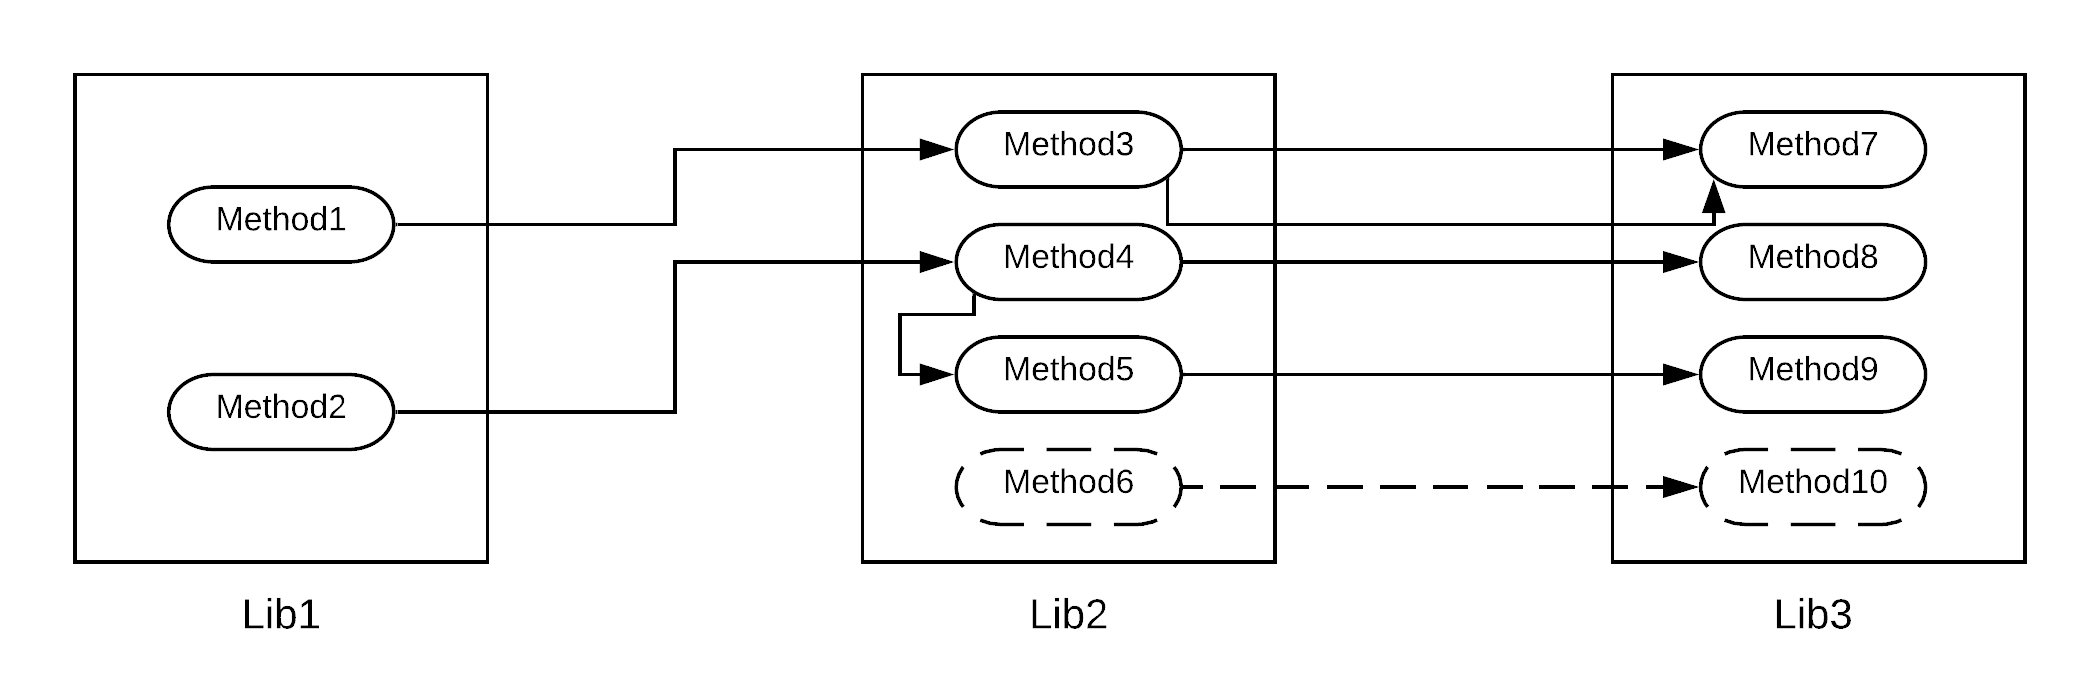
\includegraphics[width=\textwidth]{figures/Reachability.png}
\caption{Example reachability}
\label{fig:reachability}
\end{center}
\end{figure}

\paragraph{Propagation Factor}
The propagation represents how the impact of a change can spread across dependencies. In Figure \ref{fig:reachability}, a change in Method3 would affect directly the client  library (Lib1). However, a change in Method7, affects first Method3, and then it can spread to Method1, in case it is not mitigated in Method3. This possible mitigation is accounted for by the Propagation Factor.

\subsubsection{Formal definition}

\paragraph{Metric 3: Transitive method invocation coupling (TMIC)}
The metric \texttt{TMIC} calculates the method invocation coupling between a client library ($L_c$) and a server library which do not have a direct dependency. For each method in the client library ($m_c \in M(L_c)$),

\paragraph{Metric 4: Transitive aggregation coupling (TAC)}

\subsection{Theoretical validation (RQ1.5)}

\subsubsection{Transitive method invocation coupling}
\paragraph{Property 1: Nonnegativity}

\paragraph{Property 2: Null value}

\paragraph{Property 3: Monotonicity}

\paragraph{Property 4: Merging of classes}

\paragraph{Property 5: Merging of unconnected classes}

\subsubsection{Transitive aggregation coupling}
\paragraph{Property 1: Nonnegativity}

\paragraph{Property 2: Null value}

\paragraph{Property 3: Monotonicity}

\paragraph{Property 4: Merging of classes}

\paragraph{Property 5: Merging of unconnected classes}

\begin{comment}
\subsection{Defining the taxonomy of package replacement (\textbf{RQ2.2})}

Before starting the measurement of package replacement, it is important to specify which kind of replacement is being studied. Therefore, we have defined a classification of the possible scenarios.

First, Kula et al. \cite{kula2014visualizing} in their study about the visualization of the evolution of library dependency, identify four distinct behabiours. Namely, adopter, idler, updater and dropper. In addition, Kikas et al. \cite{kikas2017structure} when studying the evolution of software ecosystems, define two different types of update, explicit and implicit. Considering this two classifications, we have created the following classification:

\begin{table}[ht!]
    \begin{center}
    \begin{tabularx}{\textwidth}{|X|l|l|}
      \hline
      Description & Kula et al. & Kikas et al. \\
      \hline\hline
      Add new package dependency & adopter & - \\
      \hline
      Maintain package dependency in new application version & idler & - \\
      \hline
      Manual update of dependent package version & updater & explicit package update \\
      \hline
      Automatic update of dependent package version & updater & implicit package update \\
      \hline
      Change a dependency from one package to another & dropper \& adopter & - \\
      \hline
      Remove dependency with a package & dropper & - \\
      \hline
    \end{tabularx}
    \end{center}
    \caption{Taxonomy of depdendency evolution}
    \label{table:taxonomy-dependency}
\end{table}

\blankls
In this classification, we have added the scenario in which a dependency is dropped and substituted by another one. When looking at the terminology defined by Kula et al. it would mean dropping a package, and adopting a new one at the same time. This situation could be given due to libraries that are not maintained longer. These libraries, are usually marked as deprecated, indicating that there is no team updating it anymore. The dependencies created with these libraries, are called halted libraries \cite{pashchenko2018vulnerable}.

Vulneriabilities created by halted dependencies have to be mitigated with a different and more costly strategy. There are different options to mitigate the vulnerabilities, listed below:

\begin{itemize}
  \item Replace with a library with the same API. Therefore, the replacement would only involve changing the name of the library in the calls to it.

  \item Replace with a library in which the API is different, with different parameters needed for the calls. In this case, the replacement would involve the entire methods (units) in which the library is used.

  \item Creating a new library. The replacement of this library with this option involves developing the functionalities that were used from the original library.

  \item Contribute to the library. In this case, the effort would be related to the amount of code that needs to be changed in order to fix the bug that is causing the vulnerability.
\end{itemize}
\end{comment}
